\section{Grundlagen}



    % ######################################################################
    %     Argo-Programm
    % ######################################################################

    \subsection{Argo-Programm}

    % TODO Welche Organisationen sind beteiligt?

    Zum Ende des vergangenen Jahrtausends verdichteten sich die Hinweise auf einen globalen und durch Menschen verursachten Klimawandel. Um dessen Auswirkungen auf die Weltmeere studieren zu können, wurde unter dem Dach des \gls{GOOS} das Argo-Programm gegründet. Dieses untersucht, unterstützt durch das Satellitensystem Iason, die Wassersäule der oberen 2000m auf deren chemischen Eigenschaften. Dabei werden in ständigen Intervallen Salzgehalt, Druck, Temperatur und Leitfähigkeit gemessen. Die ermittelten Daten werden veröffentlicht, das diese durch Wissenschaftler ausgewertet werden können.

    % TODO Verweis auf die Sage der Argonauten

    \begin{figure}[h]
        \centering
        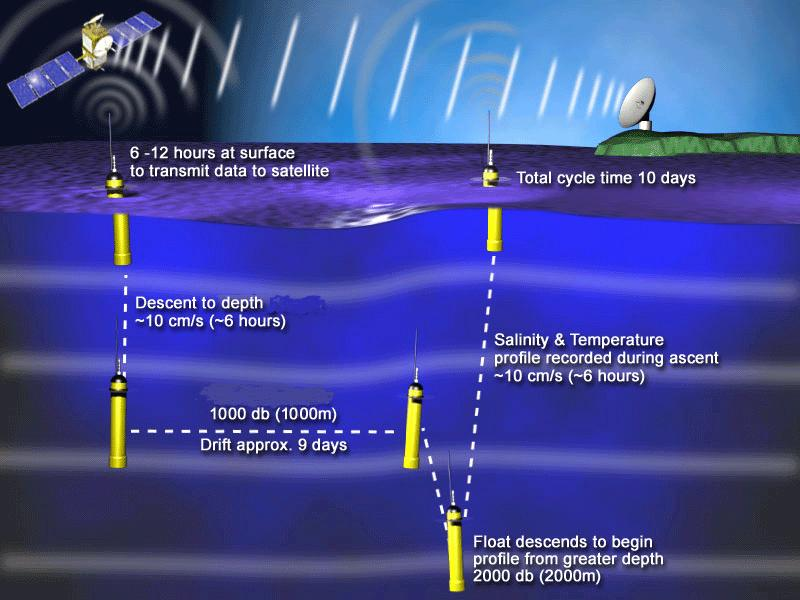
\includegraphics{pix/operation_park_profile.jpg}
        \caption[Argos Messzyklus]{Argos  Messzyklus}
        \footnotesize{
            Bildquelle: \href{https://www.csiro.au/en/Research/OandA/Areas/Marine-technologies/Argo-robotic-floats}
                        {\url{https://www.csiro.au}}
        }
        \label{fig:Argo-messzyklus}
    \end{figure}

    Die Argo Treibbojen werden mit Schiffen an spezifischen Punkten ausgesetzt. Ein Messzyklus beträgt 10 Tage. Die Boje taucht am Anfang des Zyklus auf 1000 Meter Tiefe herab.  In dieser Tiefe verbringt die Sonde die nächsten 9 Tage. Anschließend sinkt sie auf die maximale Tiefe von 2000 Metern herab, um daraufhin wieder zur Oberfläche aufzusteigen. An der Oberfläche sendet die Boje innerhalb von 6 bis 12 Stunden die Daten über den Sattelitenarray Iason an die Bodenstationen. Der oben genannte Messzyklus kann in Abbildung \ref{fig:Argo-messzyklus} nachvollzogen werden.

    \begin{figure}[!ht]
        \centering
        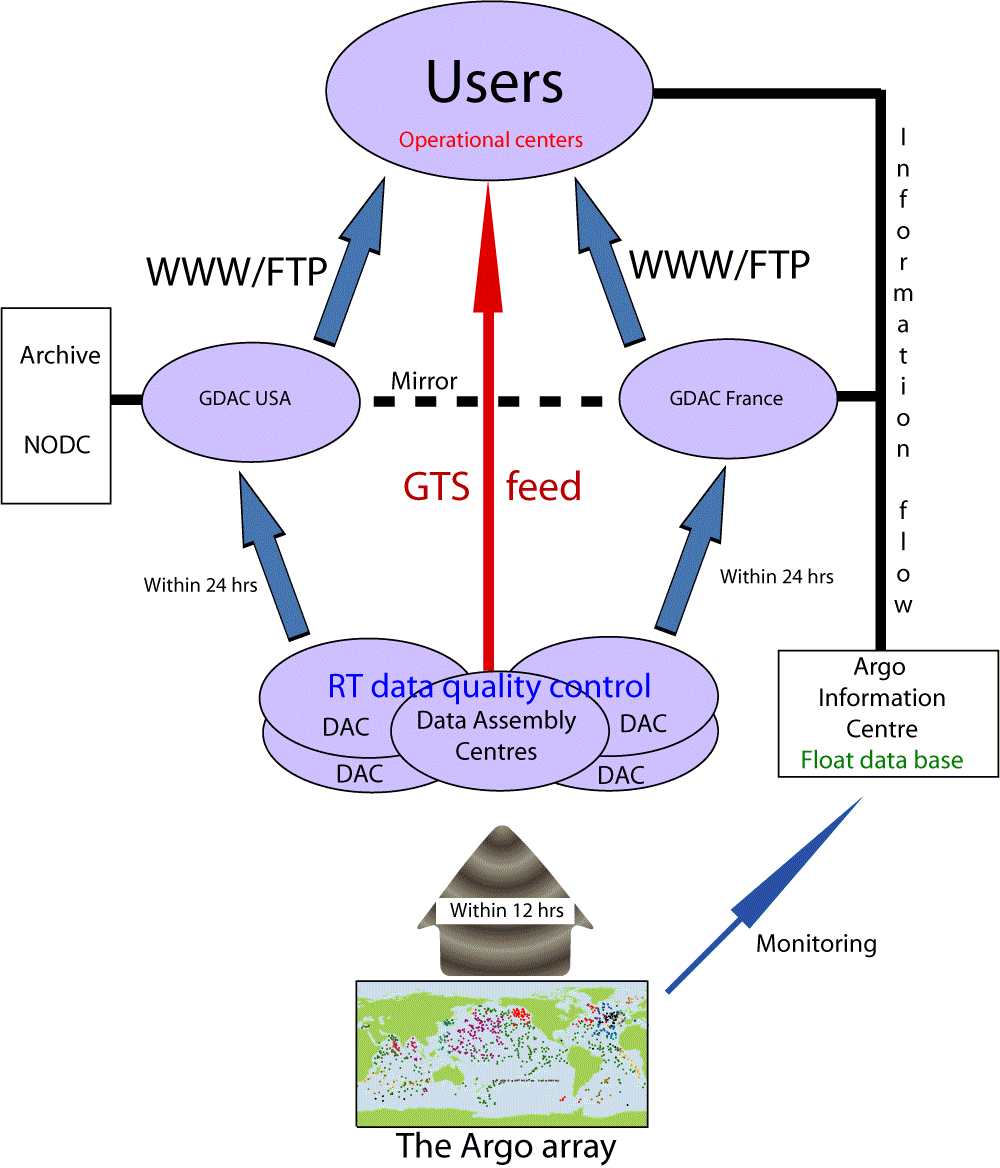
\includegraphics[width=0.4\textwidth]{pix/RT-Data-flow}
        \caption[Qualitätszyklus der Argo-Daten]{Qualitätszyklus der Argo-Daten}
        \footnotesize{
            Bildquelle: \href{http://www.argo.ucsd.edu/Argo_data_and.html}%
                        {\url{http://www.argo.ucsd.edu}}
        }


        \label{fig:argo_dataflow}
    \end{figure}

    Im Anschluss an die Erhebung werden die Daten auf deren Plausibilität und Qualität überprüft (vgl. \cite{ArgoDataBeginnersGuide} S. 3). Nach diesem Prozess werden die aufbereiteten Daten über die \gls{GDAC} in monatlichen Releasezyklen veröffentlicht. (vgl. \cite{Argofloa92:online}). Der Werdegang der Daten ist in Abbildung \ref{fig:argo_dataflow} zu sehen.

% BEGIN -- Daten
\subsection{Datengrundlage}


    Alle am Argo-Programm teilnehmenden Organisationen verpflichten sich auf eine gemeinsame Datenpolitik. So gibt es keine Herrschaft über die erhobenen Daten. Vielmehr stehen diese ab dem Zeitpunkt der Veröffentlichung transparent der Öffentlichkeit zur Verfügung.
    Nach der Übermittlung werden die Messdaten einer Qualitätskontrolle unterzogen. Sie werden auf Plausibilität und Abweichungen überprüft. Nach dieser Qualitätskontrolle werden die Daten nun über die \gls{GDAC} in Frankreich und den USA veröffentlicht. Diese können über \gls{HTTP} und \gls{FTP} abgerufen werden.

    Ein mal im Monat werden die Daten als Snapshots, unter \gls{DOI} zusammengefasst.
    Während und vor der Qualitätskontrolle liegen die Daten in den Formaten \gls{TESAC} und \gls{BUFR} vor.
    Die von den \gls{GDAC} veröffentlichten Daten liegen im Format \gls{netCDF} vor. Diese sind unter der Lizenz Attribution 4.0 International (CC BY 4.0) veröffentlicht und dürfen unter der Nennung der Lizenz frei verwendet und dabei auch verändert werden (vgl. \cite{ArgoDataDocumentation}).

% END

% BEGIN -- Datenstruktur

In Listing \ref{lst:dataOrdnerstruktur} ist die Ordnerstruktur der \gls{netCDF} Dateien zu erkennen. Über den Ordnernamen aoml ist die Herkunft des \gls{DOI} zu erkennen. In diesem Fall wurden die Dateien von einem Server der  "`Atlantic Oceanografic \& Meterolocical Laboratory"' erstellt. Hier befindet sich für jede Messboje ein Unterordner.  Die Dateien meta, prof, Rtraj und tech sind eine Quelle für Metainformationen. Die Messprofile einer Boje finden sich im Ordner \texttt{profiles}. Hier wird für jeden Messzyklus eine Datei angelegt. Dieser startet bei 1 und inkrementiert über jeden Messzyklus um 1.

    \begin{python}[label={lst:dataOrdnerstruktur}, caption={Die Verzeichnisstruktur der vom aoml bereitgestellten Daten}]
./aoml/1900200/
- 1900200_meta.nc
- 1900200_prof.nc
- 1900200_Rtraj.nc
- 1900200_tech.nc
- profiles
    - D1900200_001.nc
    ...
    - D1900200_215.nc
    - D1900200_216.nc
./aoml/1900201/
...\end{python}

% END

\subsection{Objektrelationale Unverträglichkeit}

In einem Softwareparadigma manifestiert sich ein bestimmtes Konzept in der Modellierung der Welt. Durch diese konzeptionelle Betrachtungsweise beeinflusst ein Paradigma den Erstellungsprozess sowie die Ergebnisse des Softwaredesigns und zwingt diesem seine Grenzen auf. Probleme bei der Kombination verschiedener Paradigmen werden dabei als Unverträglichkeit (impedance Mismatch) bezeichnet.
Objektorientierte Programmierung  und eine relationale Abfrage von Datensätzen sind weit verbreitete Paradigmen in der Softwareentwicklung. Damit ist die objektrelationale Unverträglichkeit eine häufig auftretende Herausforderung (vgl. \cite{ireland2009classification} S. 36-38).
Hier genannt sind unter anderem folgende Betrachtungsweisen als Ursachen für die objektrelationale Unverträglichkeit:

\begin{description}
 \item [Strukturelle Unterschiede]
 Die objektorientierte Programmierung erlaubt das Definieren beliebig komplexer Strukturen aus Methoden und Klassen. Durch Vererbungsstrukturen ist es möglich, Objekte zu spezialisieren und Grundkonzepte von Klassen zu generalisieren. Eine relationale Algebra wird durch Tupel, Mengen und Wahrheitswerte definiert. Inhärent wiederholbare Strukturen oder Hierarchien können mit diesen Mitteln nicht umgesetzt werden.

 \item [Datenkapselung]
 In der objektorientierten Programmierung können die intrinsischen Attribute eines Objektes verborgen werden. Dieses Konzept ist als Kapselung bekannt und erlaubt es, den Zugriff auf die gekapselten Strukturen einzuschränken. In einer relationalen Algebra ist eine derartige Abstraktion über die Daten nicht vorgesehen.


 \item [Objektidentität]
 Durch die Instanziierung eines Objektes aus einer Klasse erhält dieses eine eindeutige Identität. Somit unterscheiden sich zwei Objekte, auch wenn diese Träger eines identischen Datensatzes sind, durch ihre Repräsentation im Arbeitsspeicher. Relationen werden durch den Primärschlüssel, und damit über ihre Daten, definiert. Zwei eigenständige Relationen mit identischem Datensatz sind damit nicht möglich.
\end{description}


Als Hilfsmittel zur Überwindung der oben genannten Probleme werden objektrealtionale Mapper (ORM bzw. O/R-Mapper) eingesetzt. Durch dieses Mapping wird eine Schnittstelle oder Abstraktionsebene zwischen Programmteilen aus den jeweiligen Sprachparadigmen definiert, um den impedance Mismatch möglichst transparent zu überwinden.



%% TODO: Vorstellung der in SQLALCHEMY verwendeten Entwurfsmuster zur Überwindung des impedance mismatch



% BEGIN -- Geographische Informationssysteme
\subsection{Geodäsie und Kartographie}

In der vorliegenden Applikation werden geographische Daten über einen Kartendienst angezeigt. Aus diesem Grund erfolgt hier eine Zusammenfassung der wichtigsten geodätischen und kartographischen Grundlagen.


Die geographsiche Länge eines Punktes $P_l$ bezeichnet den Winkel zwischen einer vom Nullmeridian durch den Erdmittelpunkt geführten Fläche und einer Meridianebene, die durch den Punkt $P_l$ führt.
Analog dazu ist die geographische Breite eines Punktes $P_b$ der Winkel zwischen der Äquatorschnittfläche und der Flächennormalen an Punkt $P_b$ (vgl.  \cite{witte2011vermessungskunde} S. 18).
\\

Das "`World Geodetic System 1984 (WGS84)"' ist ein geozentrisches, vom Erdschwerpunkt abgeleitetes Koordinatensystem. Dieses wird unter anderem von GPS zur Zuordnung von Positionen auf der Erde verwendet. Eine schematische Darstellung ist in Abbildung \ref{fig:wgs84} zu sehen. Die  Z-Achse führt durch den Erdschwerpunkt entlang der Rotationsachse durch den Nordpol, die X-Achse vom Zentrum der Erde durch einen Nullmeridian (Greenwich) und die Y-Achse wird als Orthogonale zur X-Achse ebenso durch den Erdschwerpunkt geführt (vgl. \cite{witte2011vermessungskunde} S. 13-14).


\begin{figure}[h!]
 \centering
 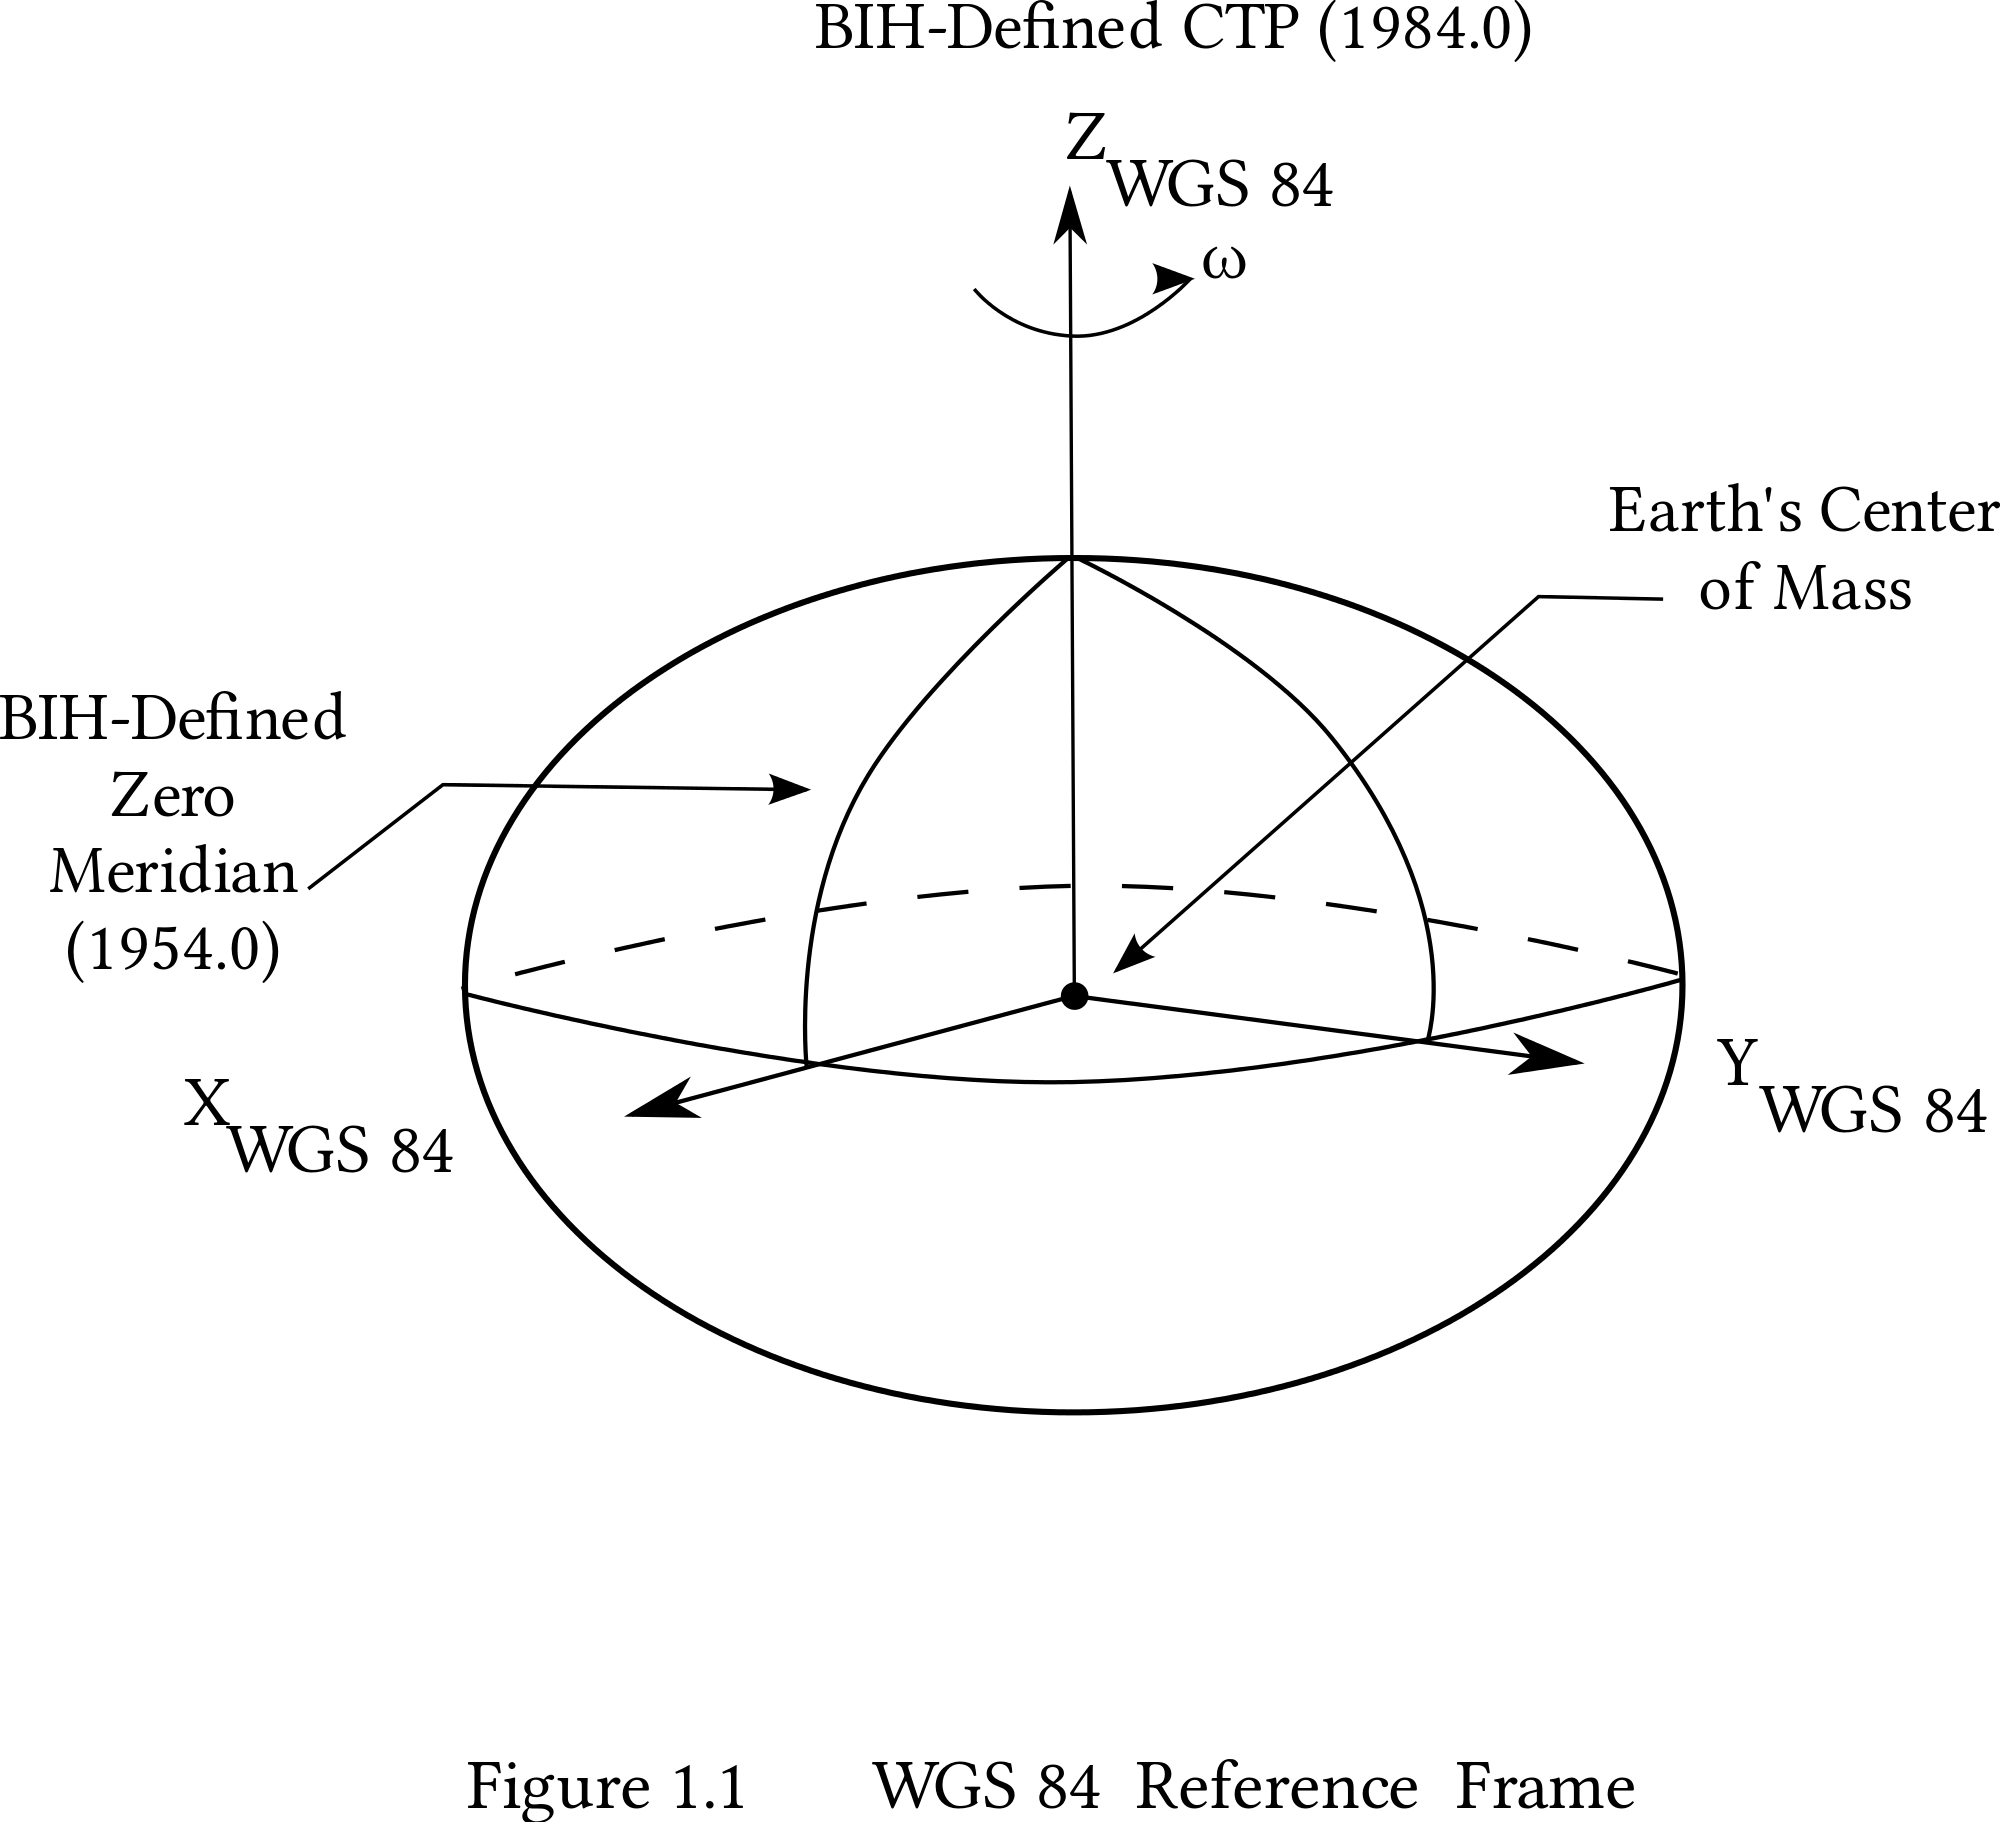
\includegraphics[width=0.3\textwidth, trim={0 9cm 0 3cm},clip]{pix/WGS_84_reference_frame.png}
 \caption[Schematische Darstellung des Koordinatensystems WGS84]
 {Schematische Darstellung des Koordinatensystems WGS84}
 \footnotesize{
    Bildquelle: \href{https://commons.wikimedia.org/wiki/File:WGS_84_reference_frame_(vector_graphic).svg}
                {\url{https://commons.wikimedia.org}}
 }
 \label{fig:wgs84}
\end{figure}



Die Gauß-Krüger Projektion erlaubt die Darstellung des Globus auf einer Ebene. Um die Krümmung des Globus auszugleichen wird die Erde in $3^\circ$ breite Meridianstreifen eingeteilt. Als Mittelpunkte dienen dabei die Meridiane $[ 3^\circ, 6^\circ, 9^\circ, \dots]$. Von den Mittelmeridianen aus wird eine Projektion an anliegende Zylinder vorgenommen. Auf diese Weise entstehen zu den Rändern der Meridianstreifen Längen- und Flächenverzerrungen, die Darstellung ist aber winkeltreu.
\\

Im UTM-System wird ein analoges Verfahren angewendet. Die Meridianstreifen haben hier aber eine Breite von $6^\circ$. Anstatt des Mittelmeridianes werden hier zwei Schnittkurven mit einem Abstand von 180km als längentreues Element für die Abbildung der Y-Achse verwendet. Der Bereich zwischen diesen Schnittkurven wird gestaucht (vgl. \cite{witte2011vermessungskunde} S. 23-25).


% END

% BEGIN -- Software
\pagebreak
    \subsection{Network Common Data Format}

    Das \gls{netCDF} dient zum Austausch von wissenschaftlichen Daten. Es ist eine Weiterentwicklung des von der NASA entwickelten \gls{CDF}. Das Datenformat zeichnet sich dadurch aus, dass es selbstbeschreibend ist. Die Dokumentation ist Teil des Datensatzes und wird so immer  mitgeführt. Dies soll die Portabilität des Datensatzes verbessern  (vgl. \cite{FishernetCDF}).

    Es wurde auch eine Bibliothek für Python entwickelt  (vgl.\cite{netCDF4}). Mit dieser ist es möglich, die Binärdaten zu öffnen und zu numpy-Arrays zu extrahieren. In Listing \ref{lst:example_netCDF} ist die Verwendung exemplarisch an der Extraktion und der Umrechnung des Erstelldatums  aufgezeigt und im Folgenden beschrieben.

    \pythonexternal[%
        % ---------------------------------------------
        %   PYTHON \gls{netCDF} als Beispiel JULD
        caption = {Extraktion eines netCDF-Datensatzes zur Berechnung des Erstellungsdatums},%
        label = {lst:example_netCDF}]%
        {scr/beispiele/netCDF_juld.py}

    Um einen Datensatz zu öffnen, bildet man eine Instanz der Klasse \texttt{netCDF4.Dataset}. Die Auswahl des Profils gelingt durch die Pfadangabe als Parameter bei der Instanzierung.
    Über das Attribut \texttt{dataset.variables} werden die Datensätze als \texttt{OrderedDict} gehalten. Bei der Extraktion eines Parameters erhält man zunächst die Dokumentation des jeweiligen Datensatzes. In diesem Fall handelt es sich um den Zeitpunkt der Sattelitenübertragung des betreffenden Messprofils.
    Aus der Dokumentation lassen sich für die Weiterverarbeitung wichtige Parameter entnehmen.
    So ist der Datensatz in Form des C-Datentyps \texttt{float64} codiert. Das Datumsformat entspricht dem \gls{Julian Day} ab dem Zeitpunkt \textit{01. Januar 1950}.

    Um die Werte eines Datensatzes zu extrahieren, wird über die numpy-slicing Operation \texttt{arr[::]} der Datensatz in vektorieller Form extrahiert. Da in diesem Array nur ein skalarer \texttt{float64} Wert enthalten ist, kann dieser als nulltes Element vom Array entnommen werden.
    Zur Überführung in das Format des Gregorianischen Kalenders wird ein Datumsobjekt des Referenzdatums benötigt. Durch die Verwendung von \texttt{timedelta} werden die Tage aus dem Feld \texttt{JULD} addiert. Da ein Messzyklus 10 Tage andauert, kann an dieser Stelle der Datensatz, durch das Überführen zu einem Integer, vereinfacht werden. Die Casting-Operation \texttt{int()} rundet in jedem Fall ab.
